Para este punto se desarrollaron nuevas instancias random distintas a las anteriores. La generación de nuevos casos de prueba es debido a que los anteriormente utilizados podrían formar una muestra aleatoria que beneficiase más a ciertos algoritmos que a otros. De esta forma podremos evidenciar diferencias entre las distintas aproximaciones.

En este nuevo conjunto de instancias se generaron $5 \times N+M$ instancias de tamaño $5 \leq N+M \leq 20$. Luego se incrementaron la cantidad de elementos de 20 a 100 tomando intervalos intervalos de 10 en 10. Para esta segunda seccion se crearon un 50$\%$ de instancias para cada tamaño.
Una vez que fueron ejecutadas todas las instancias por los respectivos algoritmos, a excepcion del backtraking el cual solo ejecuto de 5 a 15 por problemas de c\'omputo, se promedieron todas las instancias de cada tamaño para tener una mejor aproximaci\'on de las soluciones obtenidas. 

Una vez que se obtuvieron los promedios tanto de las soluciones como de la medicion de tiempo de cada algoritmo, tomamos los porcentajes de mejora, y el porcentaje de error relativo para $5 \leq N+M \leq 15$ de las heurísticas, teniendo como valor real el resultado del Backtraking.

Realizamos ciertas comparaciones para ver como se comportan las heurísticas teniendo en cuenta las conclusiones que pudimos obtener de los puntos anteriores y de esta forma obtener que heurística obtiene una mejor relación mejora de solución / tiempo.

El siguiente es un ejemplo de una instancia dentro de este conjunto nuevo, ejecutada en las 4 variantes:

  ----> Me falta hacer
    \vspace*{0.3cm} \vspace*{0.3cm}
  \begin{center}
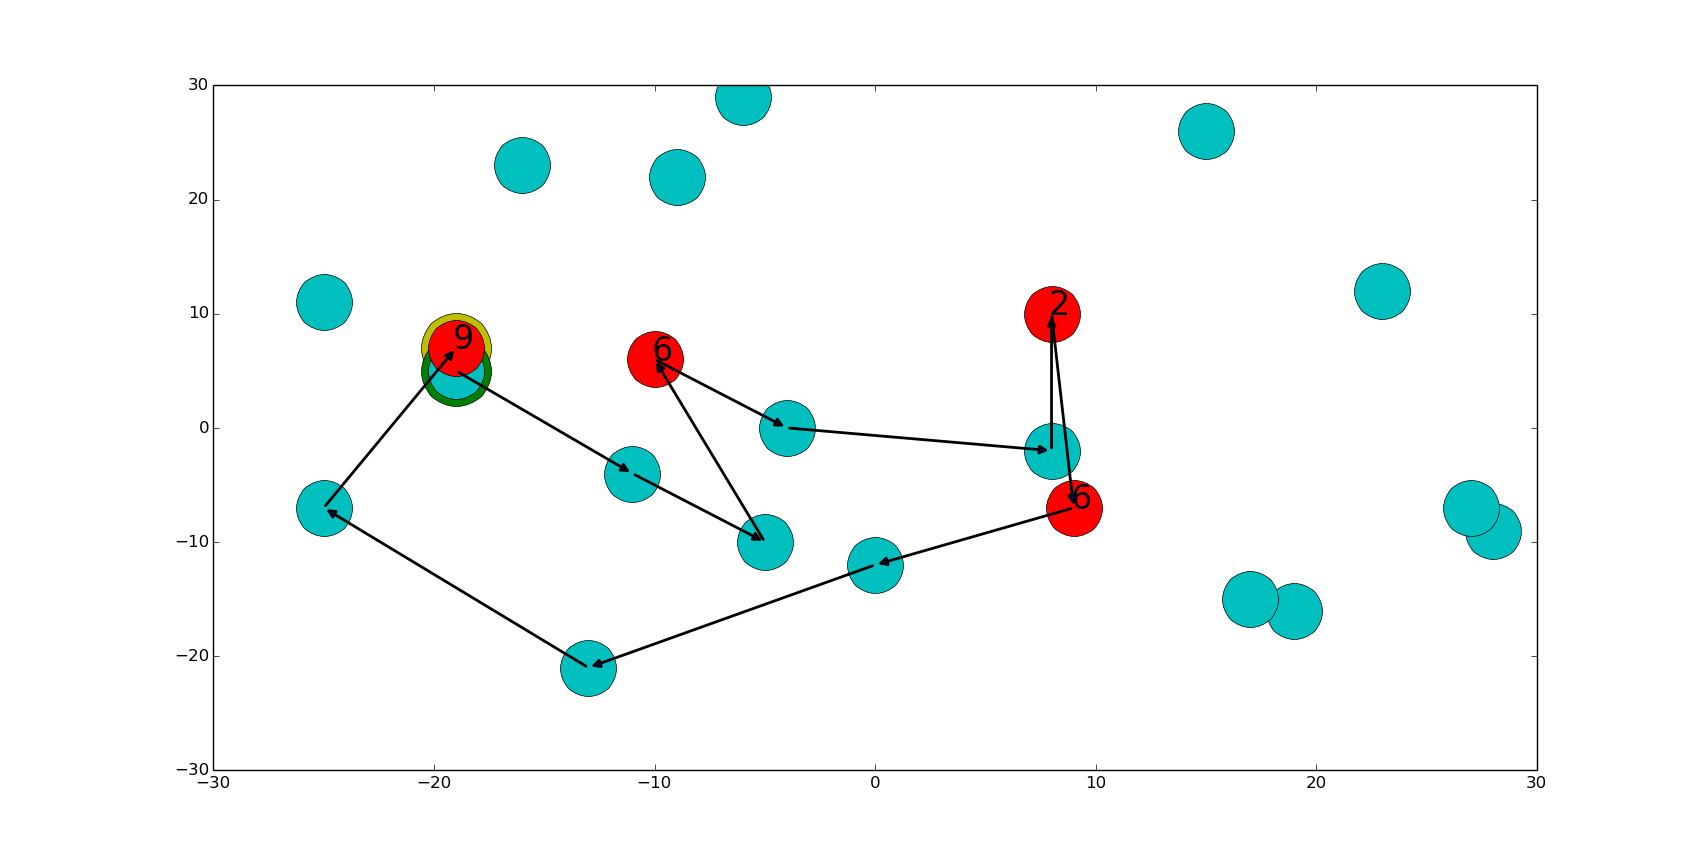
\includegraphics[scale=0.3]{./EJ5/caminoEj3opt.png}
\\{\textit{Resultado Exacto}}
  \end{center}
  \vspace*{0.3cm}

\vspace*{0.3cm} \vspace*{0.3cm}
  \begin{center}
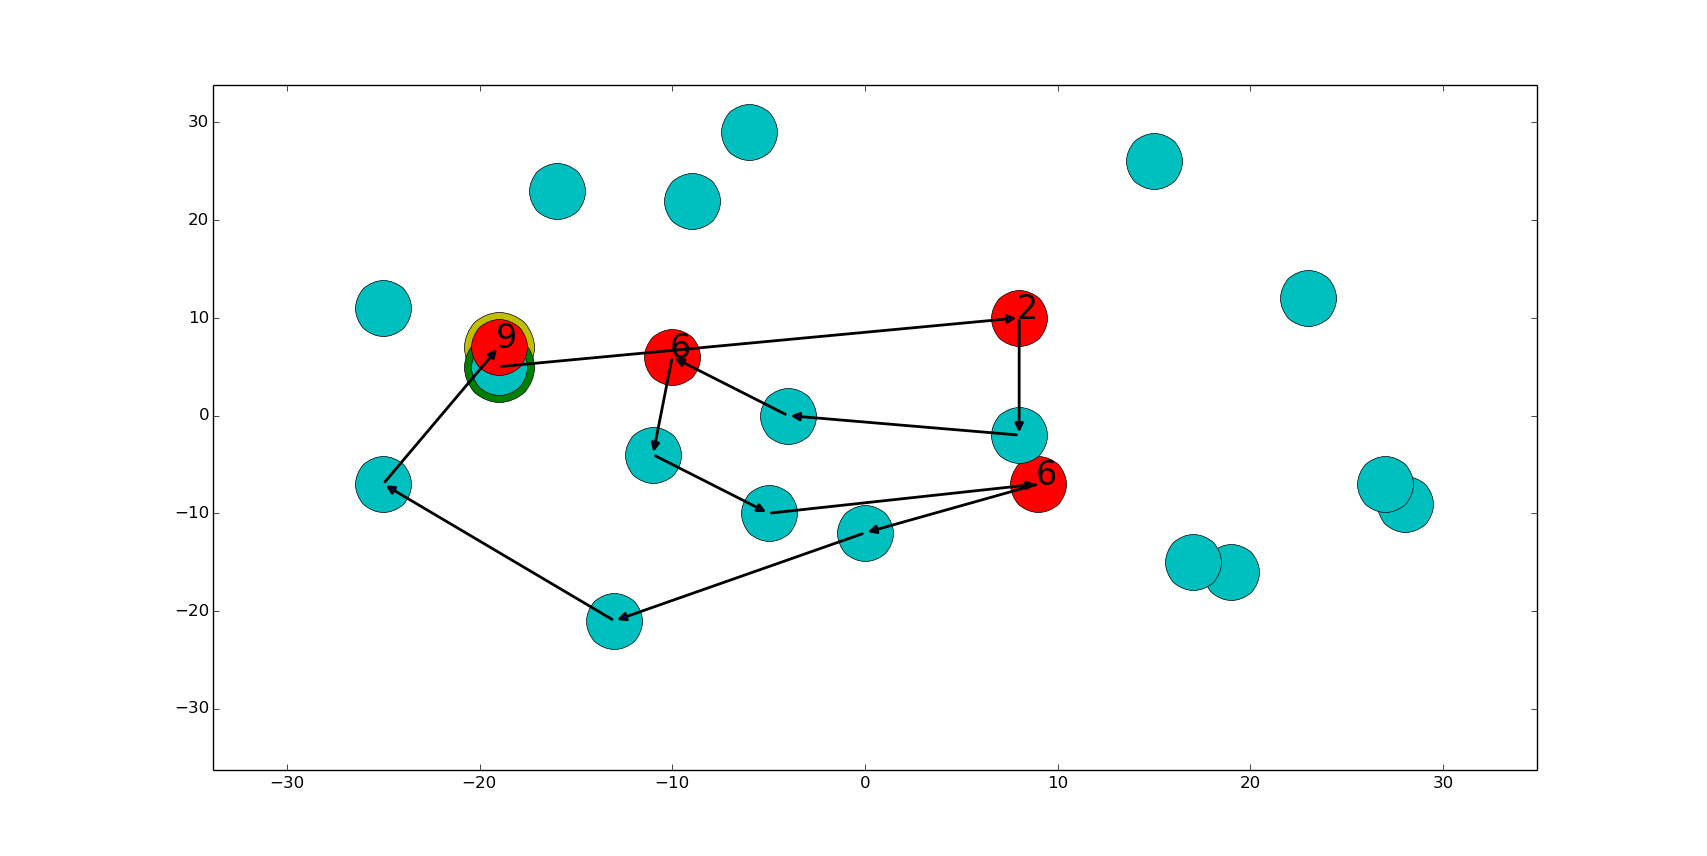
\includegraphics[scale=0.3]{./EJ5/caminoEjGoloso.png}
\\{\textit{Resultado goloso}}
  \end{center}
  \vspace*{0.3cm}
  
  \vspace*{0.3cm} \vspace*{0.3cm}
  \begin{center}
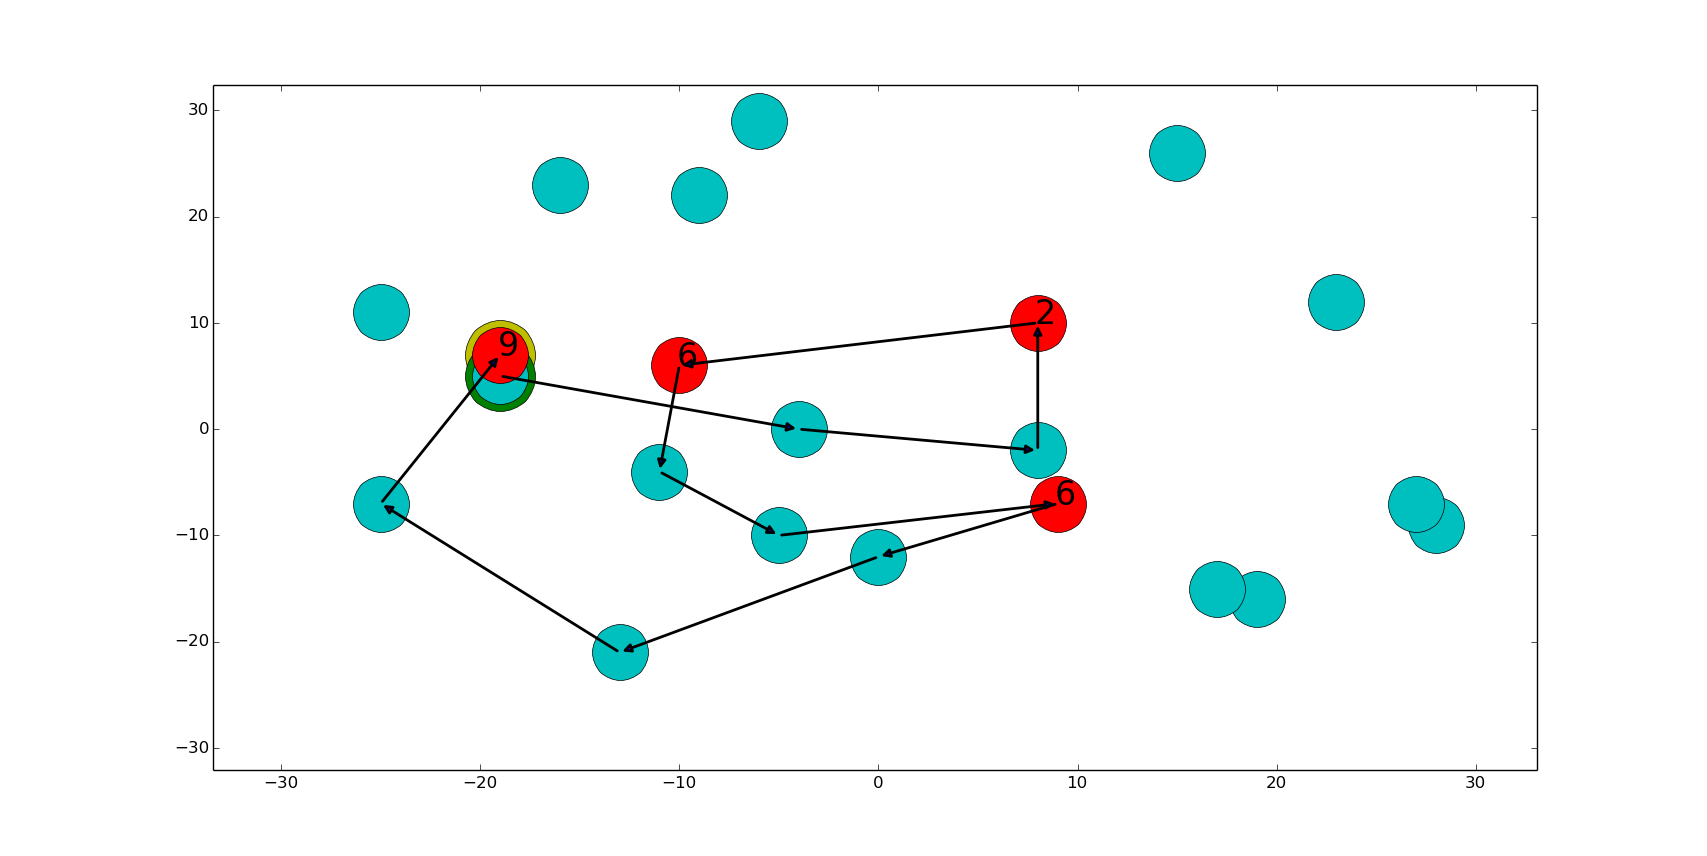
\includegraphics[scale=0.3]{./EJ5/caminoEjswap.png}
\\{\textit{Resultado SWAP}}
  \end{center}
  \vspace*{0.3cm}

  \vspace*{0.3cm} \vspace*{0.3cm}
  \begin{center}
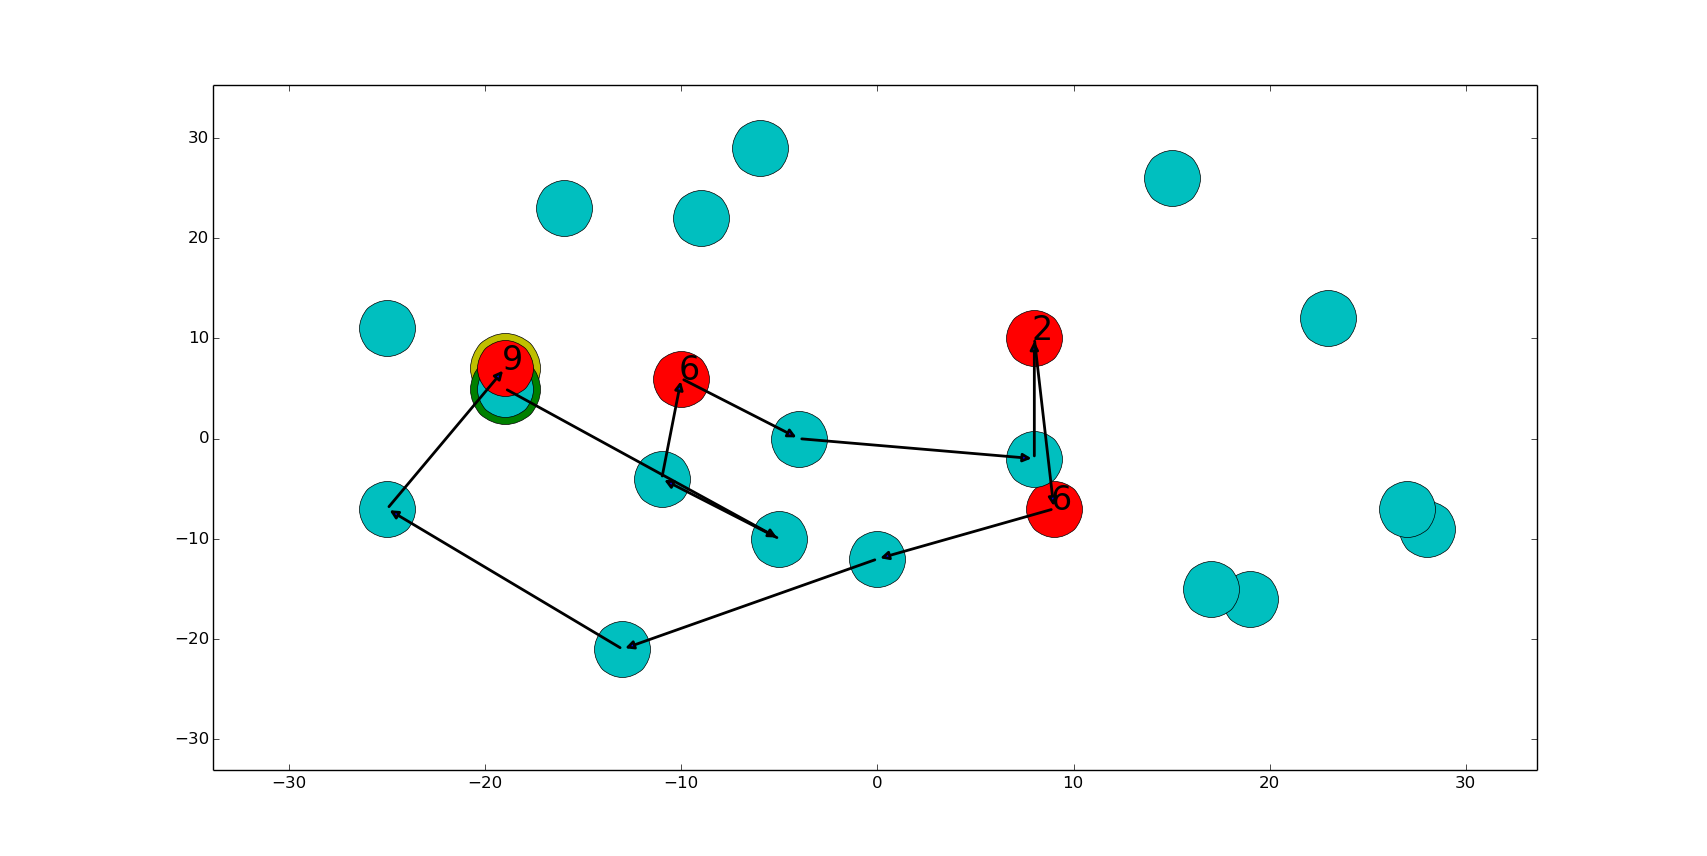
\includegraphics[scale=0.3]{./EJ5/caminoEj2opt.png}
\\{\textit{Resultado 2-OPT}}
  \end{center}
  \vspace*{0.3cm}
  
    ----> Me falta hacer
    \vspace*{0.3cm} \vspace*{0.3cm}
  \begin{center}
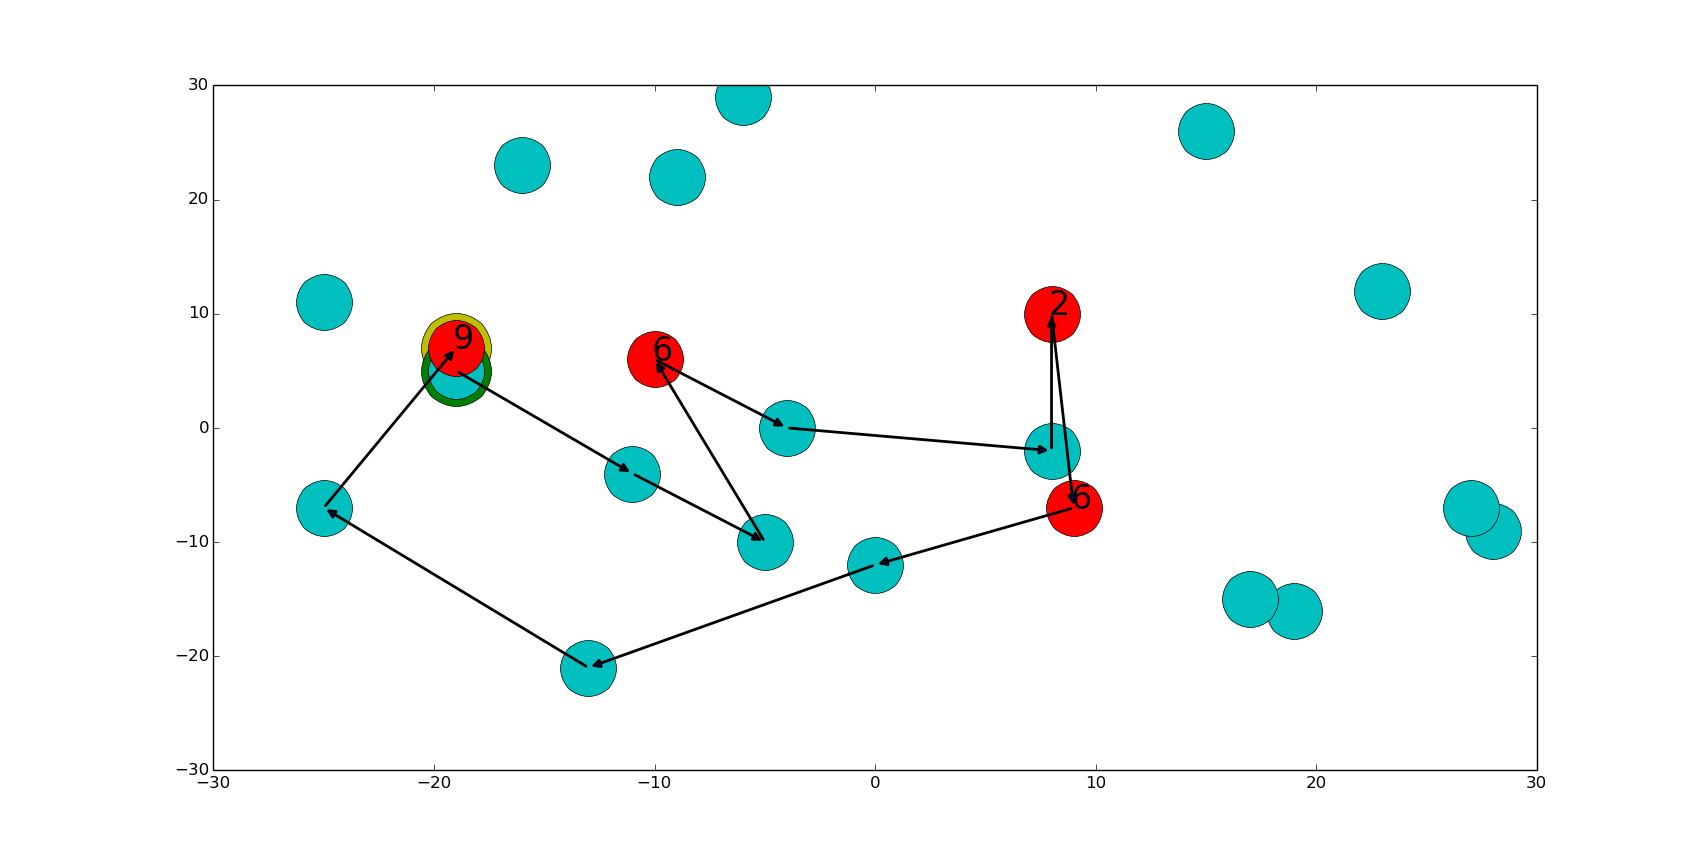
\includegraphics[scale=0.3]{./EJ5/caminoEj3opt.png}
\\{\textit{Resultado Tabu 2-OPT}}
  \end{center}
  \vspace*{0.3cm}


\subsubsection{Comparaciones de tiempo entre heuristicas}

Para corroborar la performance obtenida para este grupo de instancias se tomaron los tiempos que tarda cada algoritmo de busqueda local en obtener soluci\'on. 
 Las mediciones de las instancias de menor cantidad de elementos se compararon con la distancia exacta tomada con el backtracking. Para los casos de mayor tamaño, siendo que el tiempo de ejecución exponencial impidió la toma de mediciones, se compararon los resultados solo entre heurísticas.


\vspace*{0.3cm} \vspace*{0.3cm}
  \begin{center}
 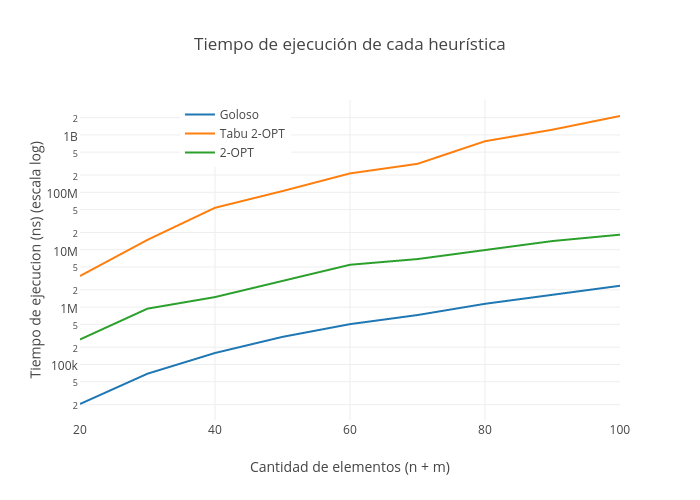
\includegraphics[scale=0.5]{./EJ5/medicion.png}\\
 {\textit{Gráfico \ 5.1 - Performance de las Heur\'isticas}}
  \end{center}
  \vspace*{0.3cm}


Podemos ver que las busquedas locales que se efectuan en menor tiempo son SWAP y 2-OPT. Las más caras son Tabú y 3-OPT. la comparación en contra de la exacta pierde sentido dada la complejidad de la misma.


\vspace*{0.3cm} \vspace*{0.3cm}
  \begin{center}
 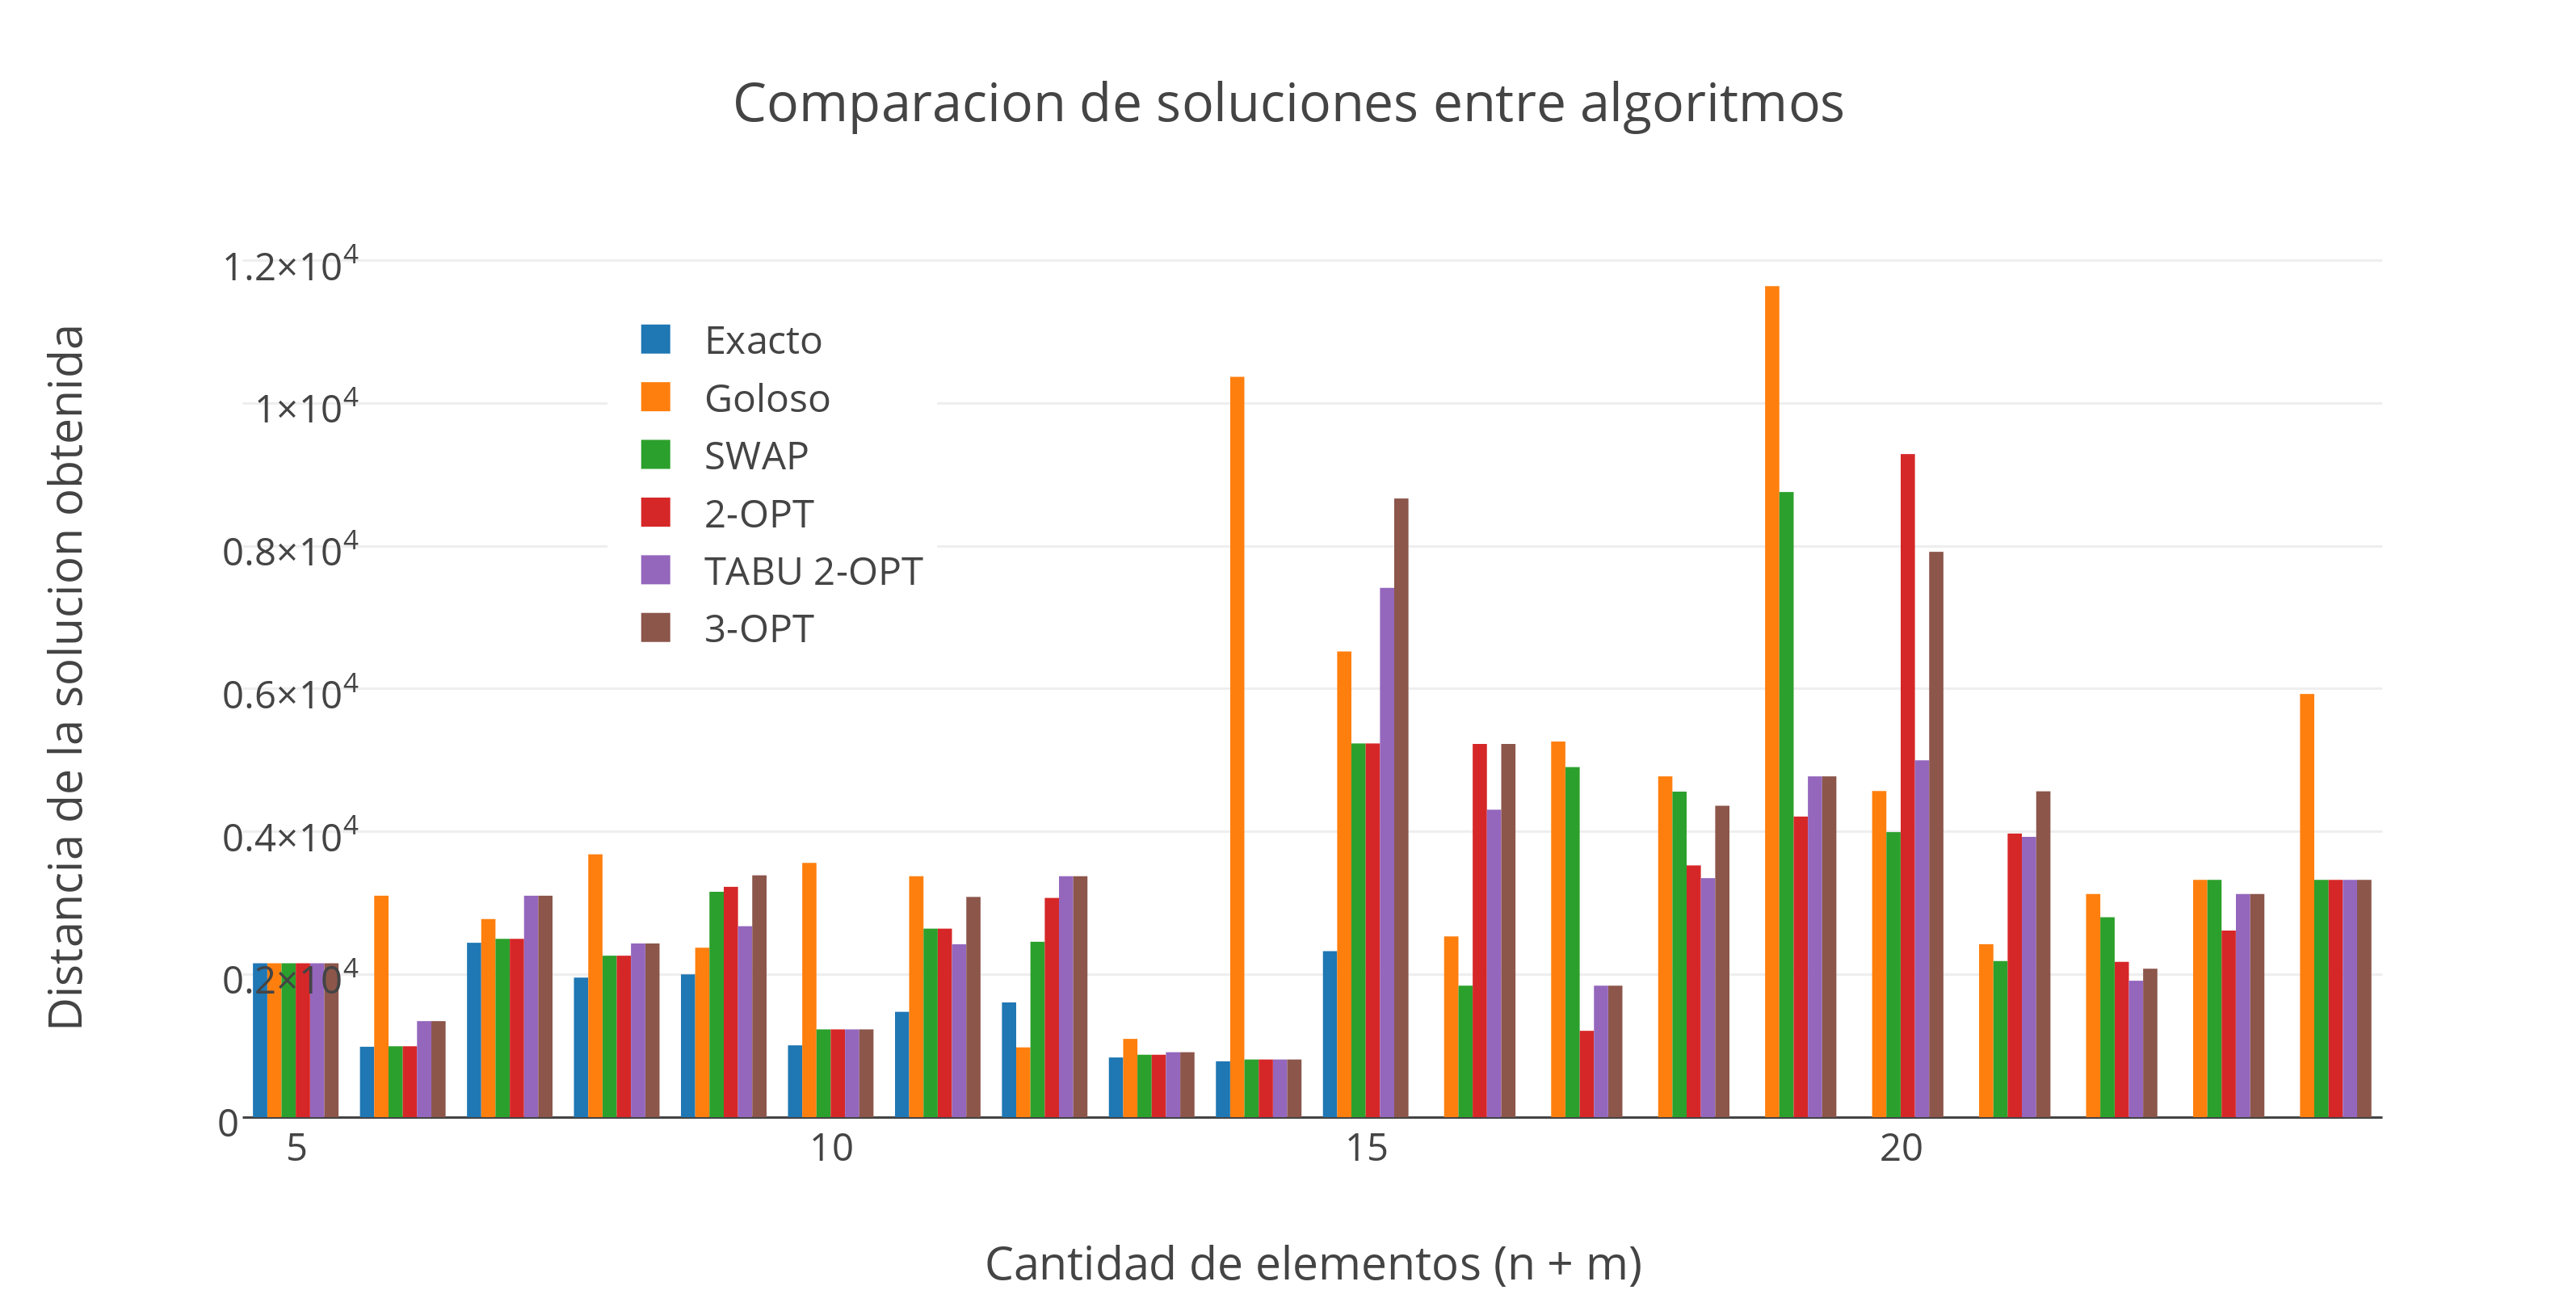
\includegraphics[scale=0.5]{./EJ5/comparativo.png}\\
 {\textit{Gráfico \ 5.2 - Comparaci\'on de soluciones de todos los algoritmos}}
  \end{center}
  \vspace*{0.3cm}
  
  


Al tener en cuenta la calidad de la solución, podemos ver que la golosa es mejorada por las búsquedas en la mayoría de los casos. En promedio las mejores las lleva a cabo 2-OPT y SWAP mientras que 3-OPT presenta el peor indice de mejora entre las busquedas locales. Por su parte, Tabú al utilizar 2-OPT, acompaña los buenos resultados de la misma e incluso, en aquellos en que el desempeño de 2-OPT no fue bueno, logra mejorarlo drasticamente (instancia de 20 elementos).
Partiendo el set de pruebas en 2, instancias pqueñas e instancias grandes, podemos observar lo siguiente:

\vspace*{0.3cm} \vspace*{0.3cm}
  \begin{center}
 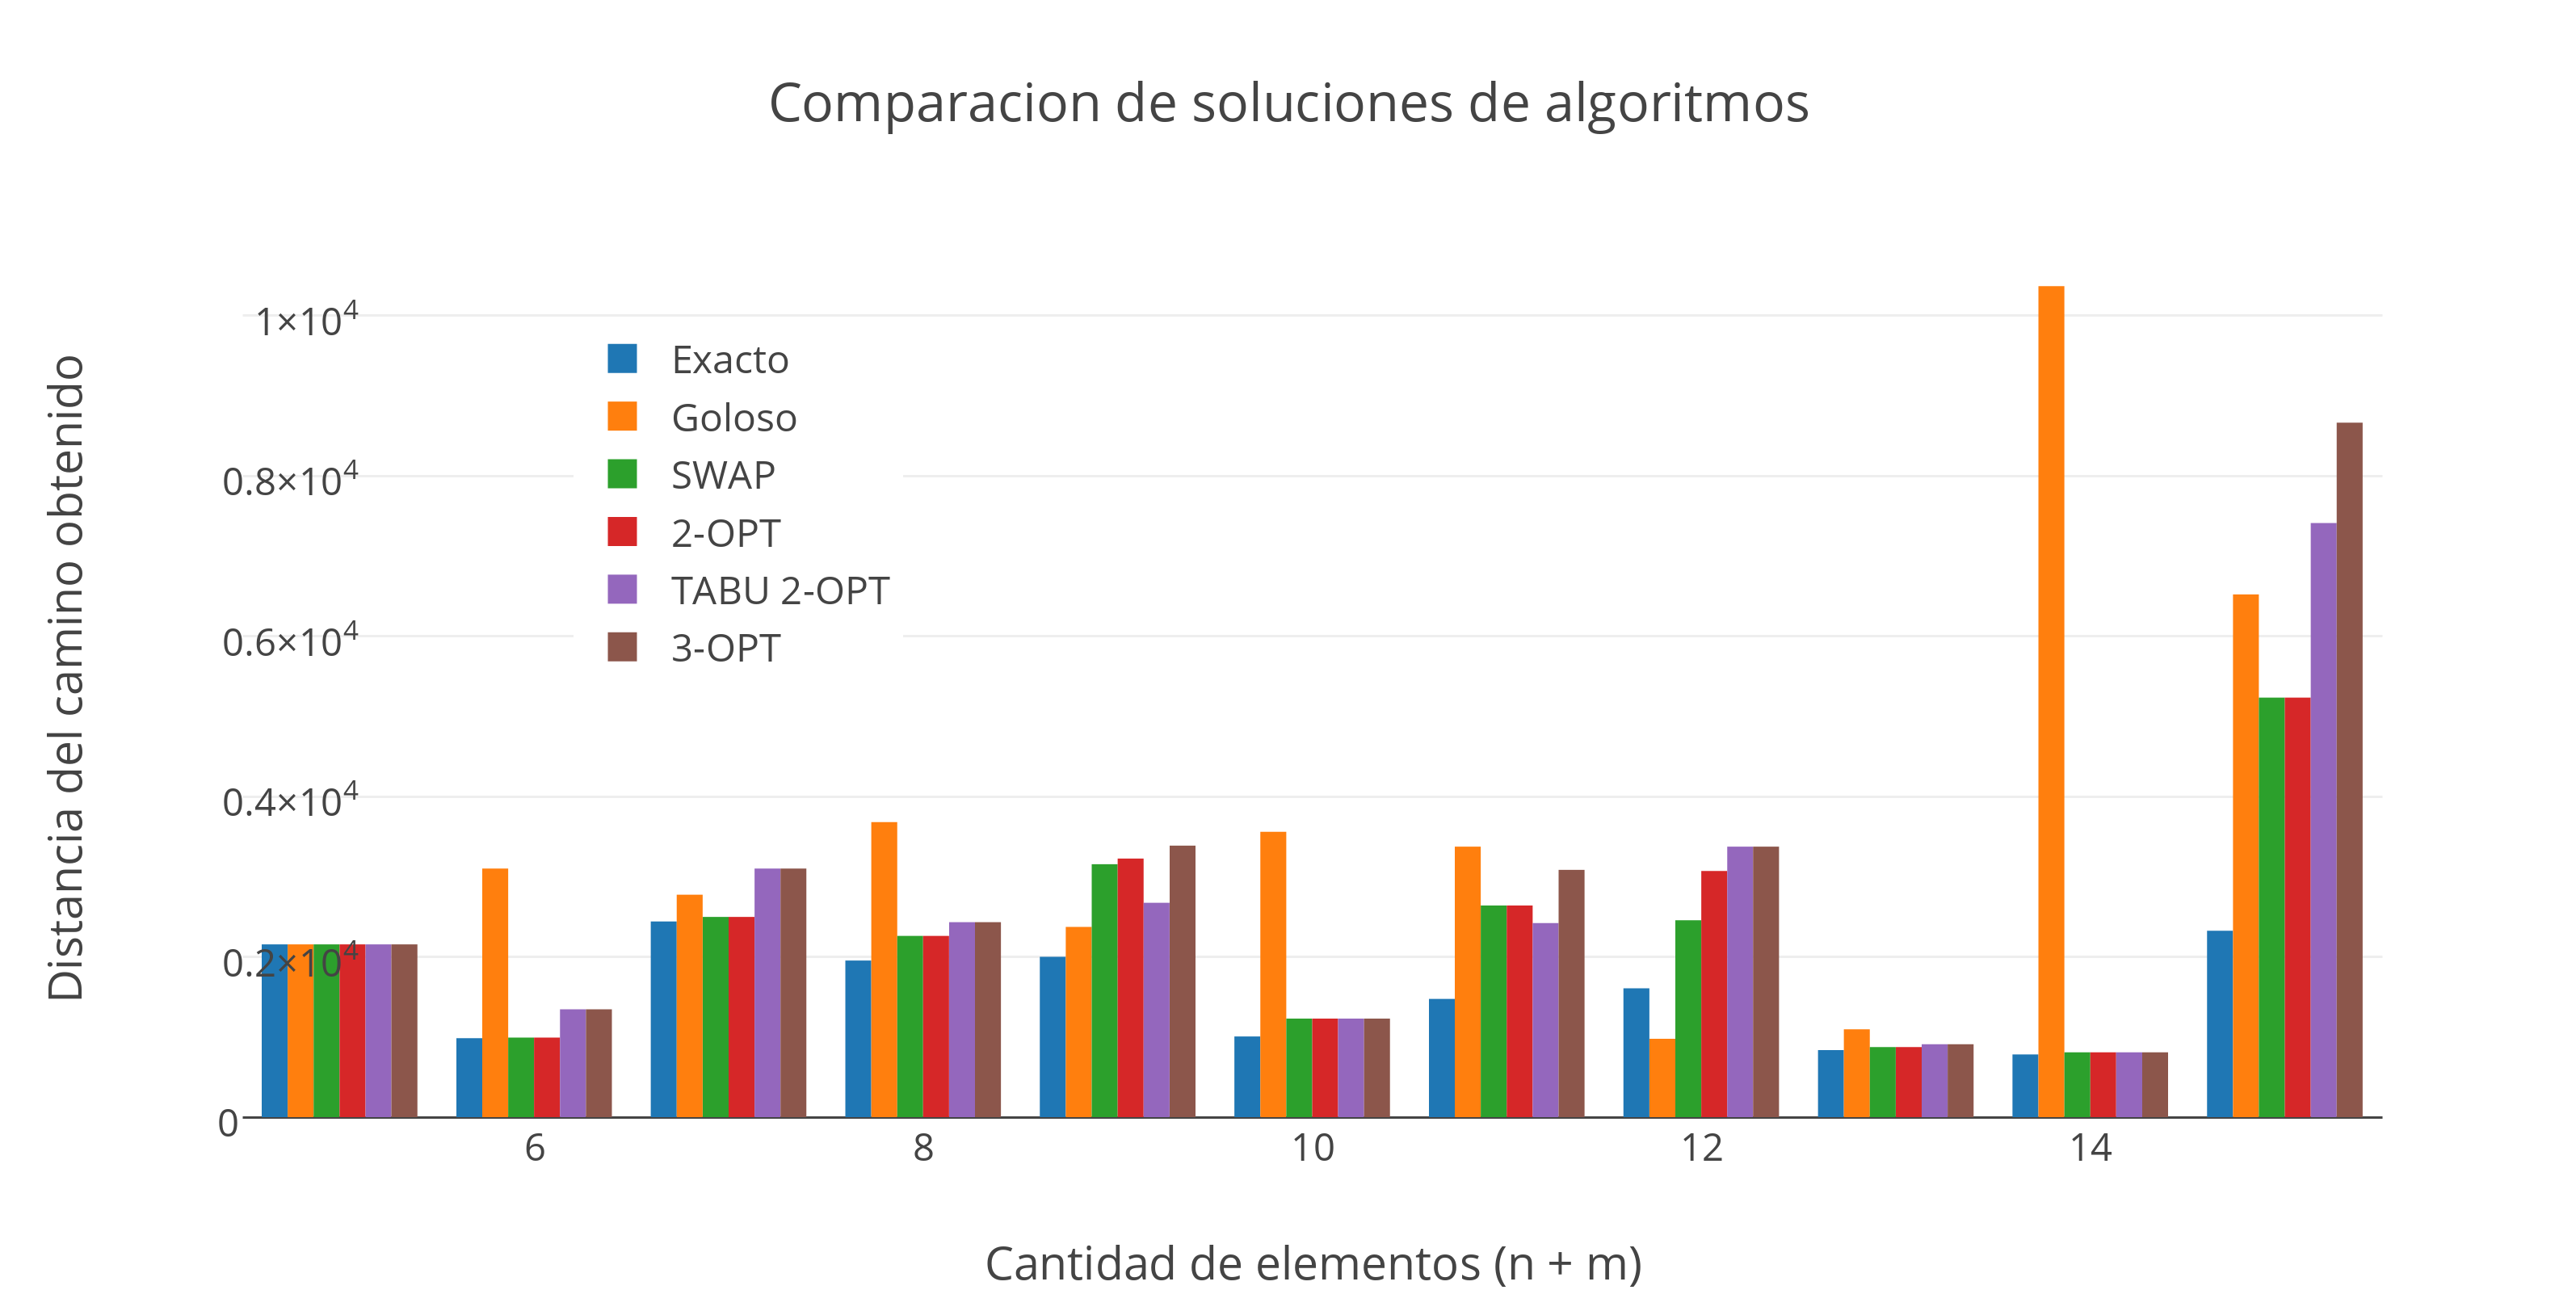
\includegraphics[scale=0.5]{./EJ5/comparativo2.png}\\
 {\textit{Gráfico \ 5.2 - Comparaci\'on de soluciones de todos los algoritmos}}
  \end{center}
  \vspace*{0.3cm}

  
\vspace*{0.3cm} \vspace*{0.3cm}
  \begin{center}
 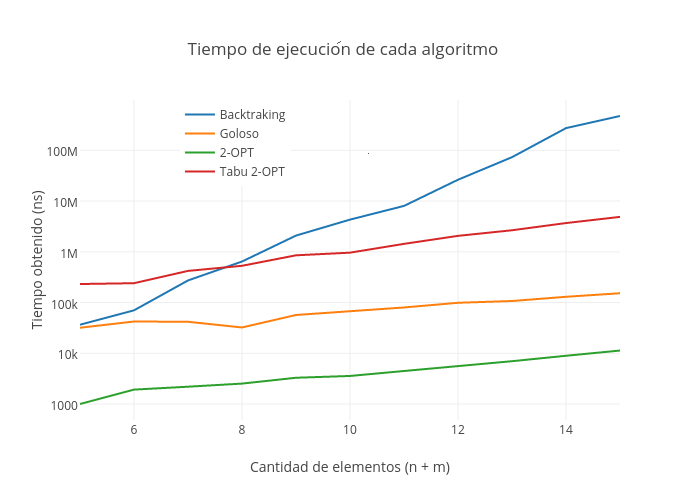
\includegraphics[scale=0.5]{./EJ5/medicionTodos.png}\\
 {\textit{Gráfico \ 5.2 - Comparaci\'on de soluciones de todos los algoritmos}}
  \end{center}
  \vspace*{0.3cm}

Las instancias de menor tamaño (de 5 a 15 elementos) producen peores soluciones al aplicarse la busqueda local que la misma heuristica golosa (cosniderando la instancia 14 como un outlier para el goloso). Lo mismo se puede observar entre 2-OPT y Tabú, en donde el segundo empeora todas las soluciones obtenidas por el primero. En cuestiones de tiempo, la utilización de Tabú pierde total sentido, ya que en aproximadamente el mismo tiempo puede obtenerse la solución exacta. Vale destacar que las mediciones de tiempo de las busquedas incluyen la ejecución del algoritmo goloso, y que en los casos en que el grafico reporta mejoras de las busquedas versus el goloso se deben a errores de medición.


\vspace*{0.3cm} \vspace*{0.3cm}
  \begin{center}
 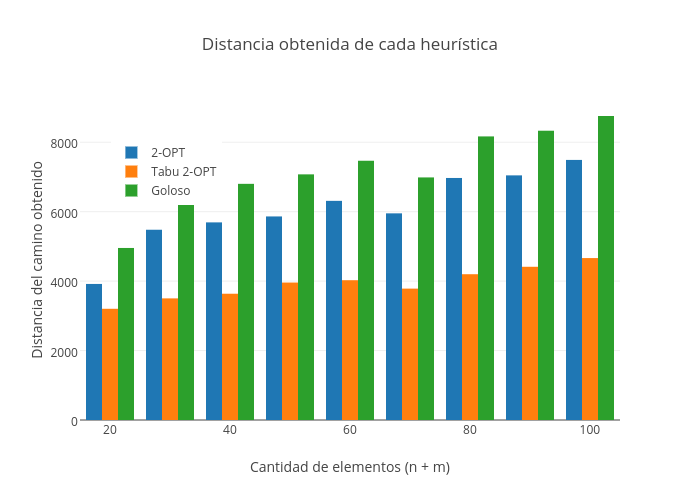
\includegraphics[scale=0.5]{./EJ5/comparativo1.png}\\
 {\textit{Gráfico \ 5.3 - Comparaci\'on de soluciones entre las heur\'isticas}}
  \end{center}
  \vspace*{0.3cm}

Al observar las intancias de mayor tamaño (de 16 a 24 elementos) podemos ver que lo anterior se invierte: a partir de la instancia 16, la solución golosa es mejorada por las búsquedas locales y las soluciones de 2-OPT, a su vez por Tabú.

\subsubsection{Comparaciones entre los errores}

Reanalizando los valores anteriormente presentados en cuanto a calidad de solución, se analizan instancias ejecutables por el algoritmo exacto. Vale notar que lo buscado es una distribución del error con menor varianza, menor mediana (es decir que el error que realice sea lo más chico posible y lo más predecible dentro de un rango determinado), y en lo posible, la mayor simetría posible: todo esto facilitaría el analisis de la solución y la predictibilidad del error mediante intervalos de confianza o la generación de estadisticos sobre las soluciones obtenidas, dandonos un mayor control y confianza sobre las mismas. la comparación entre errores que producen las heuristicas denota lo siguiente:
	
	\vspace*{0.3cm} \vspace*{0.3cm}
  \begin{center}
 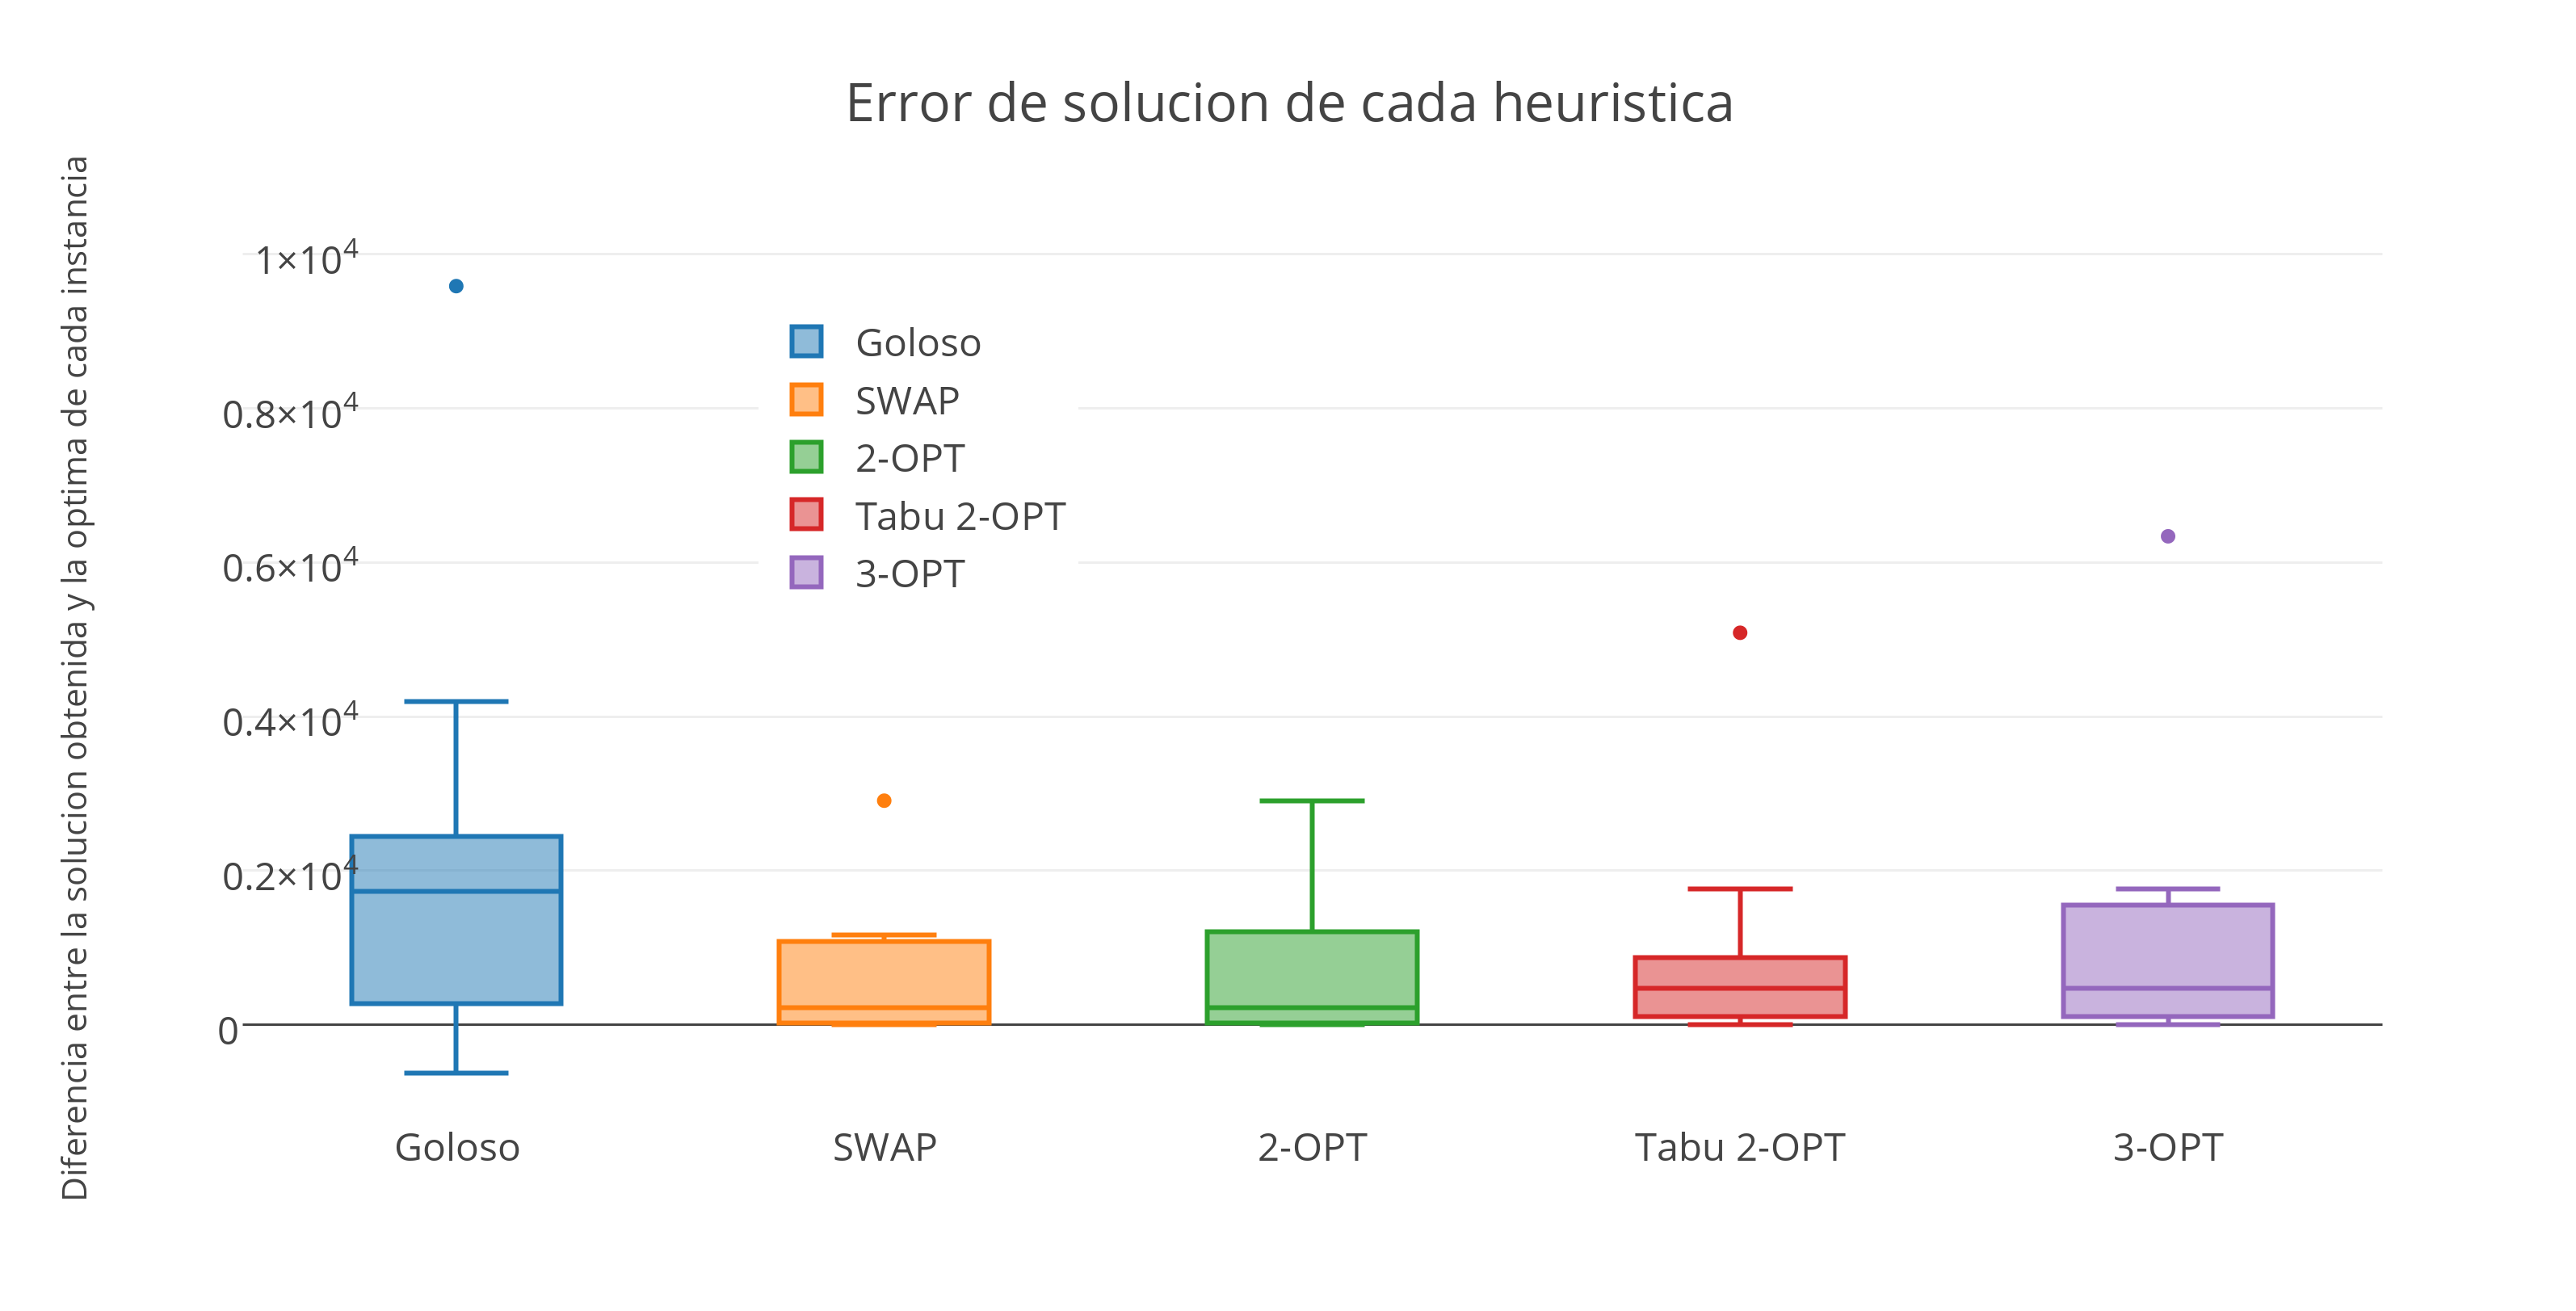
\includegraphics[scale=0.5]{./EJ5/errorporalgoritmo.png}\\
 {\textit{Gráfico \ 5.4 - Error en la soluciones de las heur\'isticas}}
  \end{center}
  \vspace*{0.3cm}
	
El algoritmo goloso es el que presenta el mayor error medio, con una varianza muy amplia en comparación al resto de los algoritmos, presenta 2 colas en la distribución del error bastante grandes. SWAP por su parte, mejora ampliamente la variabilidad del error del goloso: disminuye determinantemente las colas de la distribución y decrementa el error medio, que en comparación con 2-OPT es apenas menor. Siendo Tabú implementado con 2-OPT, se puede observar que mejora a distribución del error de éste, de forma que su distribución pasa a ser preferible a la de SWAP, ya que presenta menor varianza y más simétría, mejorando las colas de la de 2-OPT. Finalmente la aproximacion mediante 3-OPT produce los peores resultados, con la mayor variabilidad y mediana del error.


\subsubsection{Concluciones}

La resolución de ciertos problemas a nivel exacto se tornan impracticables a partir de cierto tamaño del problema a analizar, con lo cual es necesario sacrificar exactitud, por obtener al menos una solución. Al intentar solucionar este problema mediante heuristicas, se recae en el hecho de que, dado que no se tiene idea de cual es la solución buscada, es necesario obtener cierta "confianza" de las soluciones que se puedan llegar a obtener.

Al experimentar con la heuristica golosa, pudimos ver que su comportamiento lo podemos mejorar mediante la aplicacíon de busquedas locales, las cuales nos permitieron aumentar notoriamente la confianza de la solución obtenida: algunas heuristicas de busqueda, no obstante, fueron descartadas ya que  su costo/beneficio era muy alto en comparación a la del mismo méotodo goloso (Refiriendonos a 3-OPT). 

Tanto la busqueda mediante SWAP como 2-OPT nos brindaron los mejores resultados. La base de 2-OPT de Tabú nos permitio incluso mejorar lo anteriormente logrado, siendo de esta forma la metodología preferida, en cuanto a calidad de solucion. No obstante, de no contar con tanto tiempo de cómputo, la decisi\'on se deberá llevar a cabo entre SWAP y 2-OPT, las cuales se empatan bastante en calidad vs. tiempo.\\

\textbf{Experimentaciones a realizar de interés}\\
Dado que 2-OPT y SWAP obtuvieron resultados muy similares y que se implementó Tabú con el primero, es de interés desarrollar el mismo también en base a SWAP y poder realizar comparaciones entre las 2 impementaciones para poder observar su comportamierto y las diferencias que surgen entre ambos, buscando un mejor error.

